
\subsubsection{Action Suggestions}

This part of the application is designed and developed not only with the goal to provide users with actionable suggestions for household energy conservation in an easily accessible way, but also to facilitate the process of voluntary behavior change such that this process can be adapted and followed up (e.g. with one-minute use) by users in the busyness and competing priorities of their everyday life. 

A list of about fifty actions\footnote{\url{https://goo.gl/R11QdZ}} is composed to provide accurate information about actionable suggestions in the behavoir change process towards energy conservation. It is a pool of concrete household energy conservation actions based on information from credible sources such as reputable national and international energy agencies and associations. Many suggestions selected are micro-actions that are practical and inexpensive to implement in everyday life, including one-time actions such as \textit{Use energy efficient cooktops}, routine actions such as \textit{Line dry, air dry clothes whenever you can}, as well as in-between actions (reminders) such as \textit{defrost your fridge regularly (in $x$ days)}. Each suggestion has a short description, accompanied by a simple explanatory note, and the corresponding effort entailed and the estimated impact (on a five-point scale). Figure \ref{fig:actions}-(1) shows an example. The action suggestions are tailored to the local (i.e. Trento and Stockholm test sites) context when needed by local project partners, reviewed by user groups, and translated into the local languages. 

By way of caveat, some suggestions enlisted may seem obvious and trivial, but this does not mean that users are indeed doing them in practice. The goal of the design is to facilitate the behavior change process to bridge the attitude-behavior gap, making energy conservation actions new habits integrated in everyday household practices. 

The action suggestions composed are not meant as prescriptions for what users should do for energy conservation, but to present users different ideas of what they can do and how to do it in common household practices. The users are offered with a pool of actionable options which they can freely choose from according to their own context. This line of thought in design is reflected in the way the information is framed and conveyed to the users. 

\begin{itemize}
\item With the YouPower application, a user can follow a few energy conservation actions at a time. Each user has an overview (the \textit{Your Actions} tab) of his/her own current, pending, and recently completed actions. Figure \ref{fig:actions}-(2) shows an example. 
\item A new/next action suggestion is presented to the user when an old/previous action is completed, or when the user wishes to add an action (by clicking an \textit{Add Action} button). 
\item When prompted with a suggestion, the user can decide whether to take the action, or indicate that he/she is alreading doing it or the suggestion is not applicable to his/her situation. Figure \ref{fig:actions}-(1) shows an example. (The four options are: I already do this consistently; I want to do this; I don't want to do this; this doesn't not apply to me.) 
\item After a suggested action is accepted, the user may postpone (i.e. reschedule), abandon or indicate that the action is completed. Figure \ref{fig:actions}-(3) shows an example. (The three options are: I have done this consistently; I want to postpone this action; I don't want to do this anymore). 
\item When an action is pending (i.e. scheduled), e.g. \textit{defrost your fridge in $x$ days} ($x$ is set by a user), it will be triggered by time so that the application reminds the user of the pending action. 
\item In application settings, the user can choose whether to repeat a completed action, reconsider a declined action, or reassess if an action is applicable to the user.
\end{itemize}
\begin{figure}
\centering
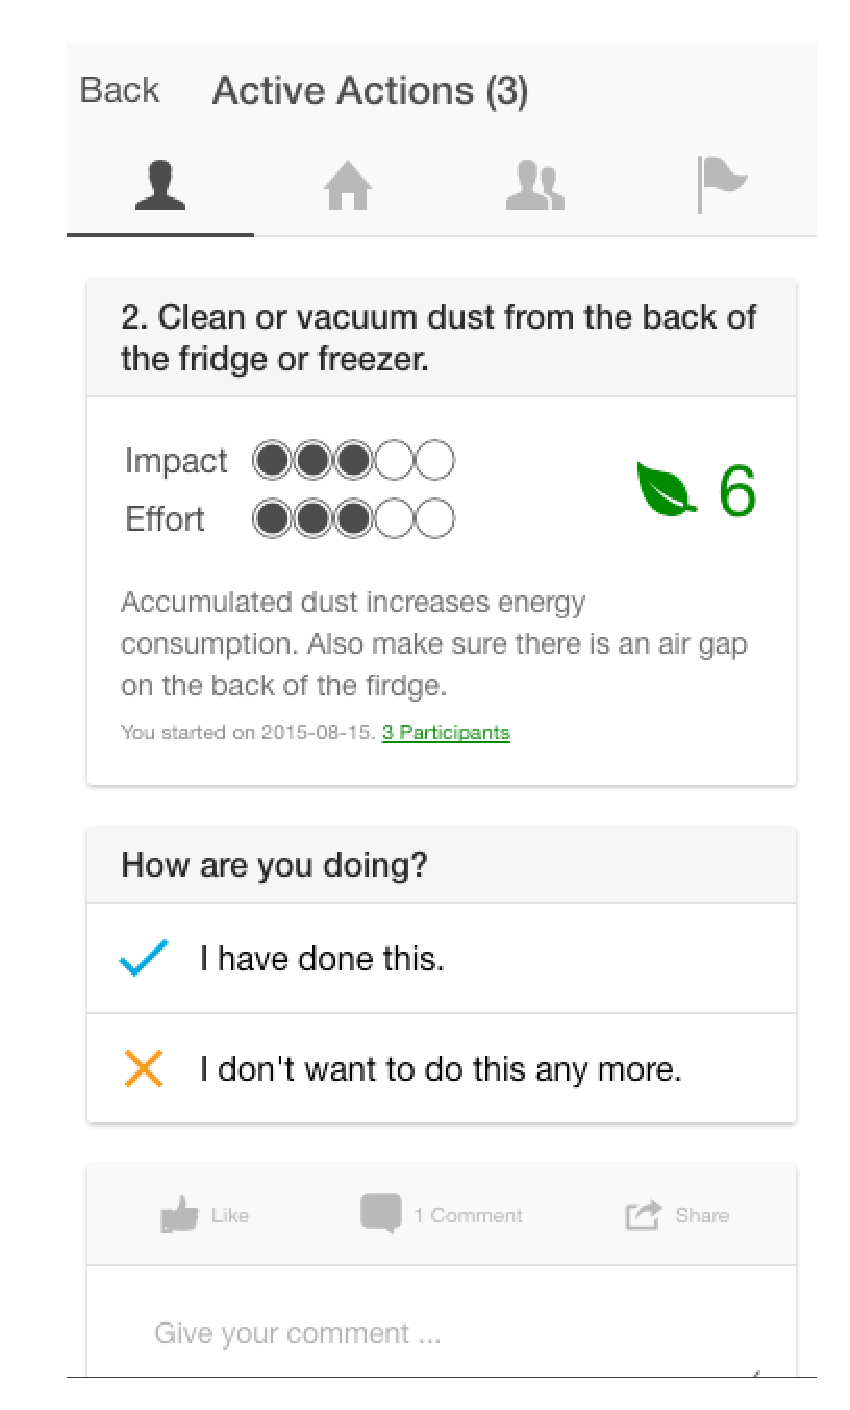
\includegraphics[width=0.33\linewidth]{img/action_details}
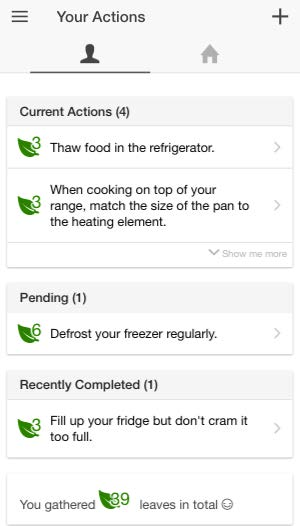
\includegraphics[width=0.33\linewidth]{img/action_tab}
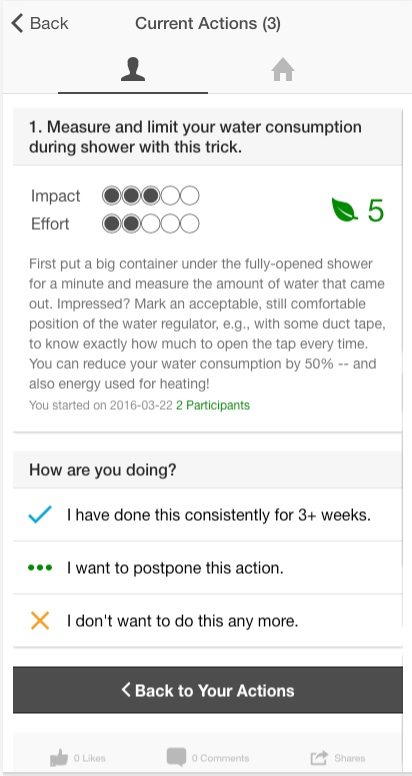
\includegraphics[width=0.307\linewidth]{img/Your_Actions.jpg}
\caption{(1) An action suggestion; (2) User actions tab; (3) An action in progress
}
\label{fig:actions}
\end{figure}

The YouPower application also uses a number of other design elements to promote users' motivation and engagement in the behavior change process. In principle, the focus is placed on providing supports for relatedness, competence and autonomy, promoting pro-environmental and altruistic values, and making one's energy conservation actions and commitments more publicly observable. 

\begin{figure}[t!]
      \begin{center}
        \begin{minipage}[t!]{0.4\linewidth}
	       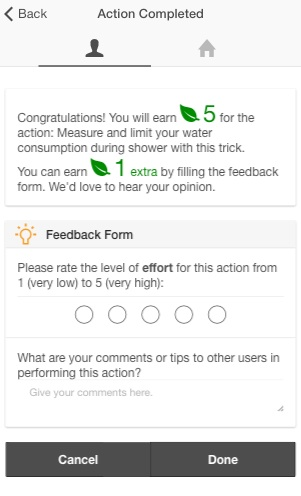
\includegraphics[width=1\linewidth]{img/action_completed.jpg}
           \vspace{2.75cm}
        \end{minipage}
        %\hfill 
        \begin{minipage}[t!]{0.4\linewidth}    
         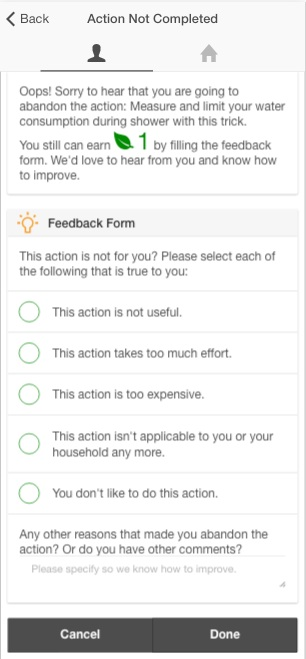
\includegraphics[width=1\linewidth]{img/action_not_completed.jpg}    
        \end{minipage}
      \end{center}
      \caption{Feedback form when a user (1) completes, or (2) abandons an action}\label{fig:form}
\end{figure}

\begin{itemize}
\item Each action has points (displayed as \textit{Green Leaves}) associated to the effort and impact score of that action. If a user completes an action, the user is awarded with leaves.
\item A user can like (with a \textit{Like} button) and comment on the actions (which are visible to all users). After a user completes or abandons an action, the user is asked to provide feedback (to the YouPower team). Figure \ref{fig:form} shows examples. The user is awarded with leaves if he/she gives comments and feedback (1 leaf each). 
\item The application encourages users to take small steps and gives them positive performance feedback. For example, when a user is taking up many actions, the application can prompt that \textit{You already have $x$ actions in progress. You can add more actions after some of those are completed. Keep on! You are doing great.} 
\item A user can signup and login YouPower with a Facebook account. If so, the user can ``share'' an action on Facebook. Figure \ref{fig:share} shows an example. 
\item The users are presented with the information about how many users have been taking an action (including Facebook friends when logged in through Facebook). 
\item A user can configure a personal profile and household profile.
\item A user can add members to his/her household; Figure \ref{fig:house}-(1). If so, the user can see the actions of household members; Figure \ref{fig:house}-(2), and add the actions to his/her own action list.
\item A user can send friends Email invitations to join YouPower (Figure \ref{fig:invite}).
\end{itemize}

\begin{figure}
\centering
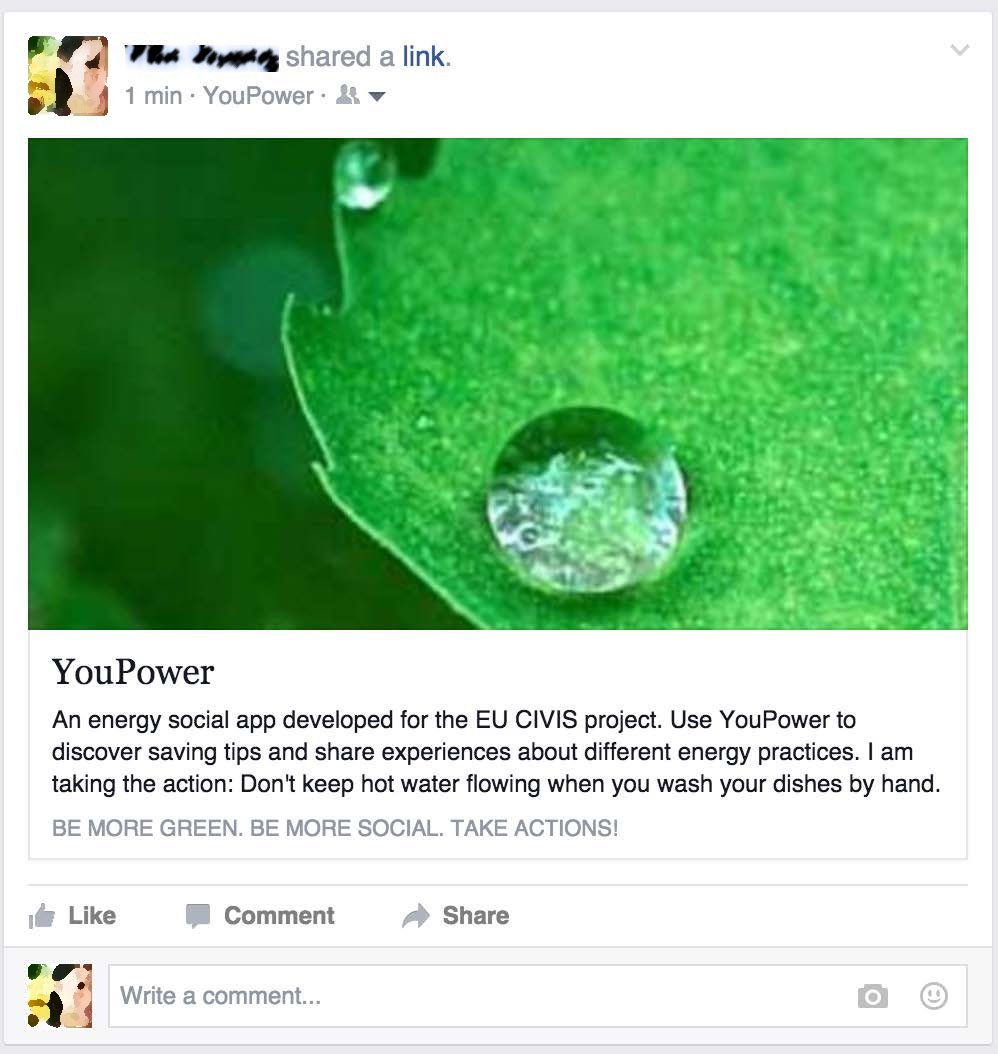
\includegraphics[width=0.62\linewidth]{img/share}
\caption{Facebook share of a YouPower action}
\label{fig:share}
\end{figure}

\begin{figure}[t!]
      \begin{center}
        \begin{minipage}[t!]{0.3\linewidth}
	       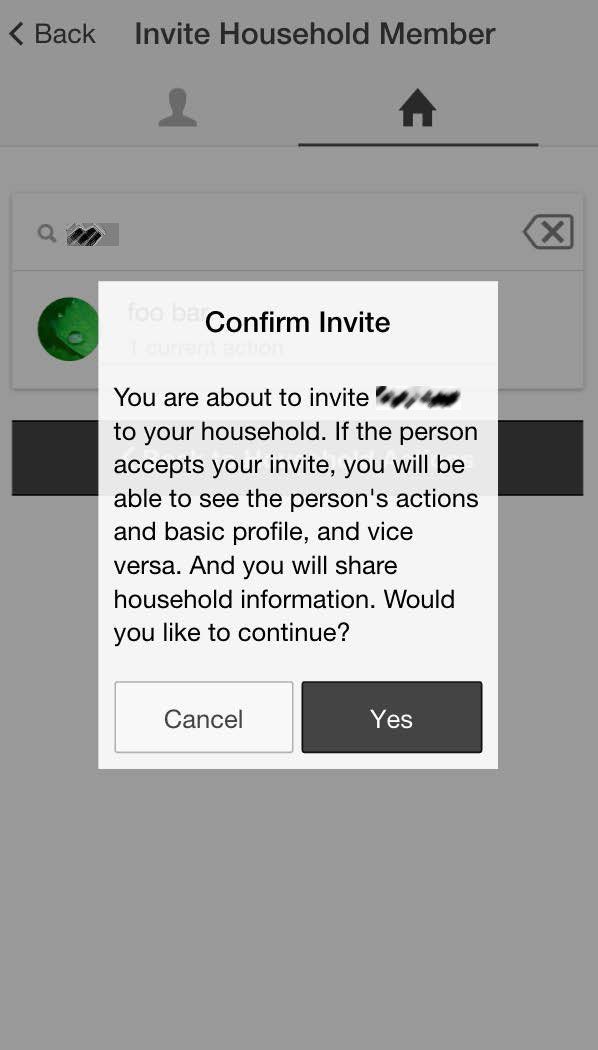
\includegraphics[width=1\linewidth]{img/house1.jpg}
        \end{minipage}
        %\hfill 
        \begin{minipage}[t!]{0.3\linewidth}    
         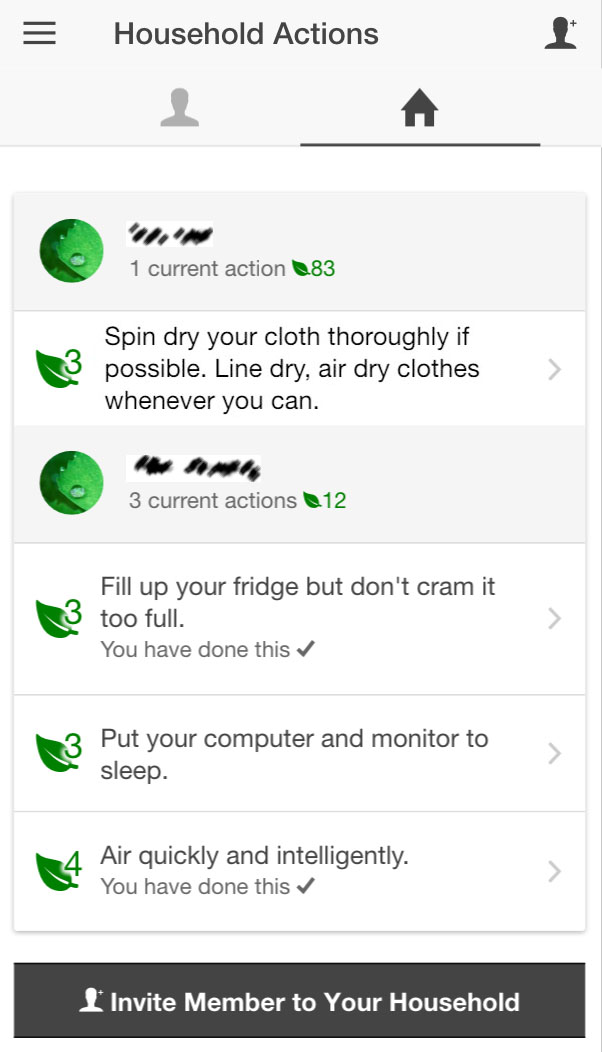
\includegraphics[width=1\linewidth]{img/house2.jpg}    
        \end{minipage}
      \end{center}
      \caption{(1) Invite household member; (2) Household member actions}\label{fig:house}
\end{figure}

\begin{figure}[t!]
      \begin{center}
        \begin{minipage}[t!]{0.3\linewidth}
	       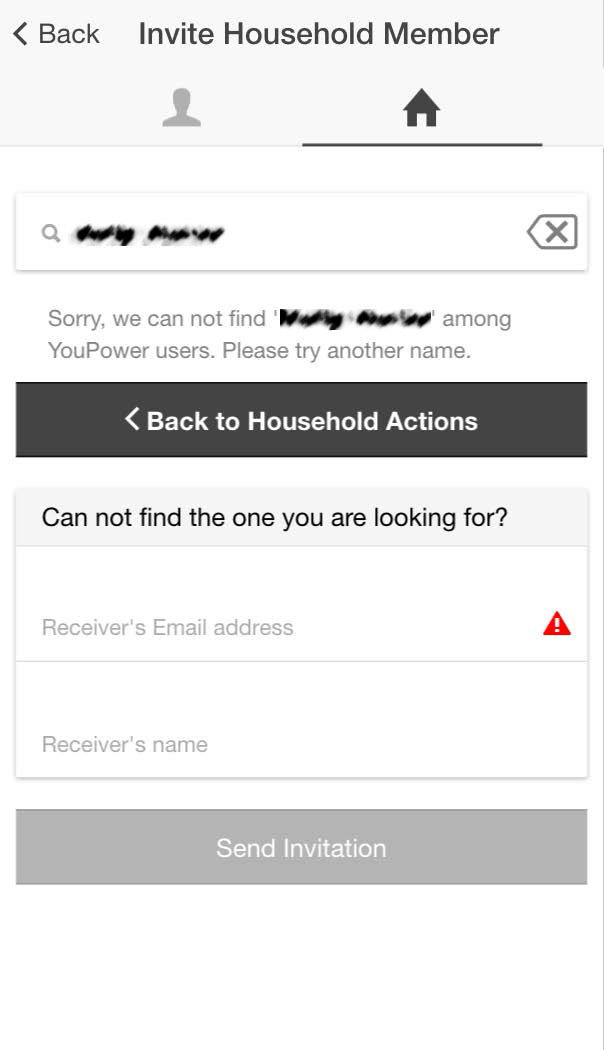
\includegraphics[width=1\linewidth]{img/invite1.jpg}
        \end{minipage}
        %\hfill 
        \begin{minipage}[t!]{0.65\linewidth}    
         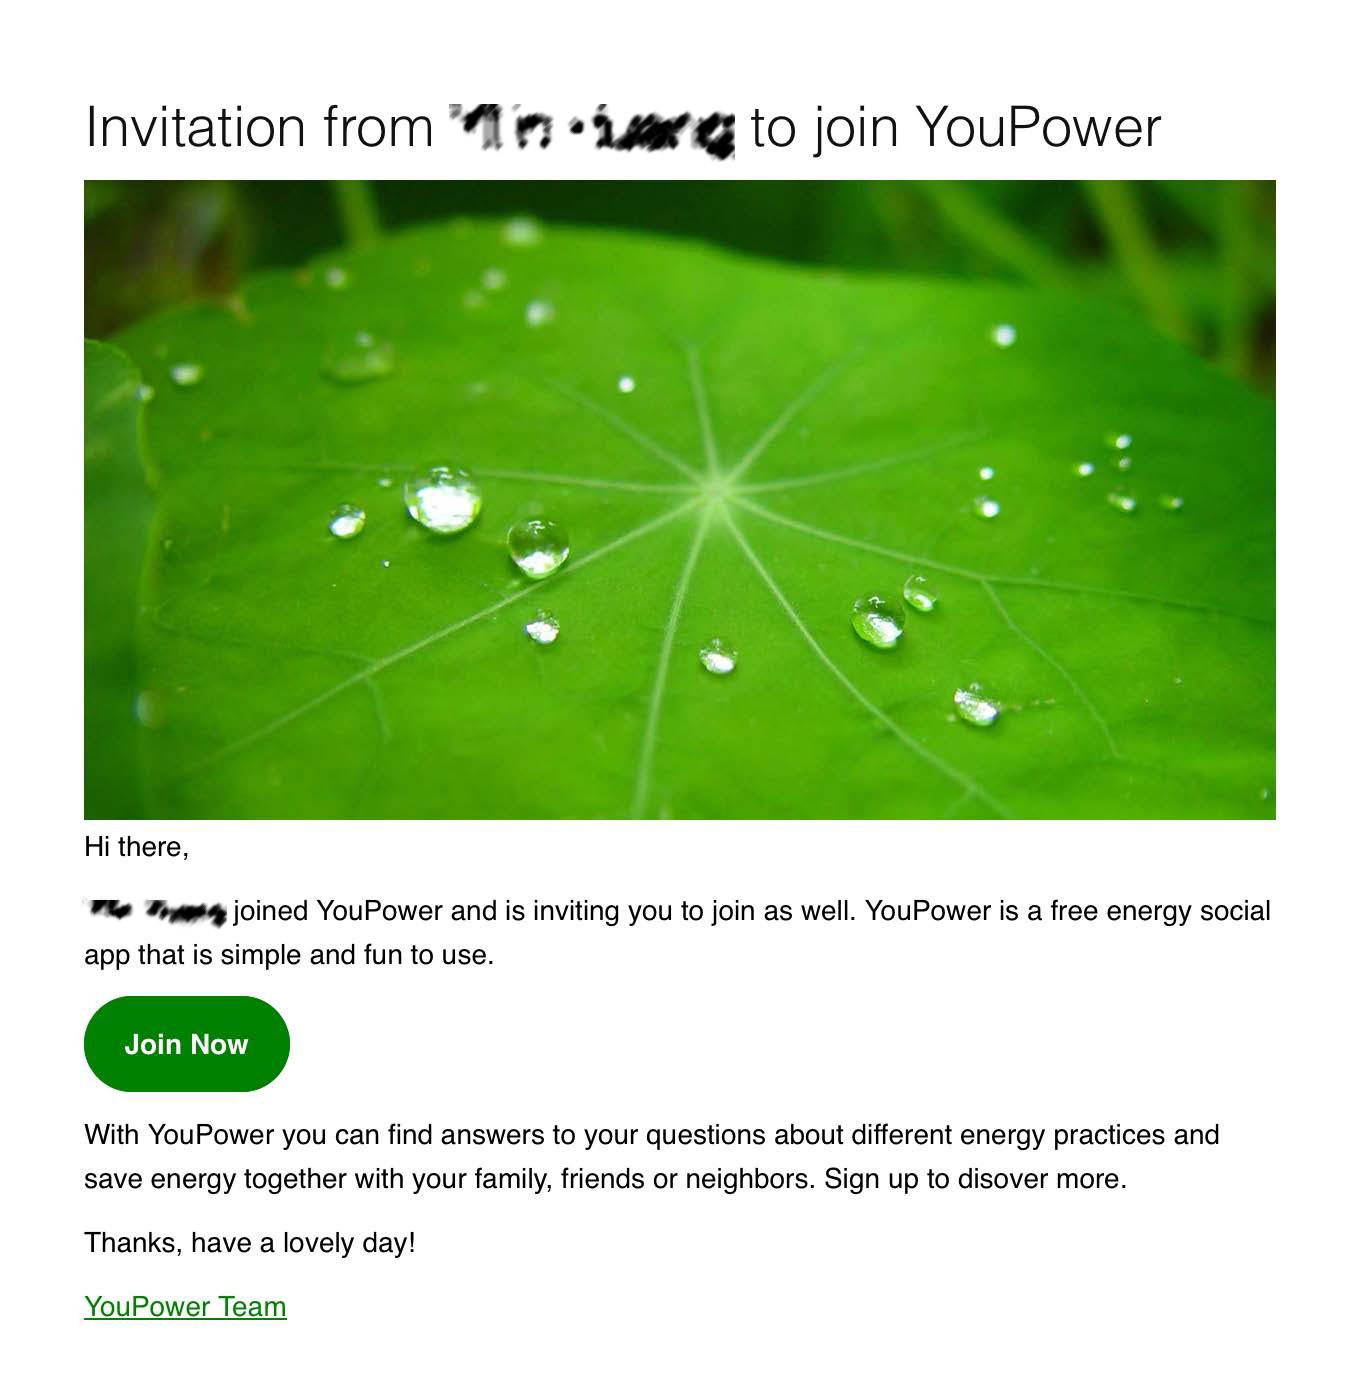
\includegraphics[width=1\linewidth]{img/invite2.jpg}    
        \end{minipage}
      \end{center}
      \caption{Send Email invitation to join YouPower }\label{fig:invite}
\end{figure}

The intention of the design (besides those already mentioned) can be highlighted as follows. For the options of choosing actions, see e.g. Figure \ref{fig:actions}-(1) and Figure \ref{fig:actions}-(3), first person narrative (e.g. \textit{I don't want to do this}) is used to create a personal micro-environment for the user \citep{Crumlish2009} to have a moment of self-reflection on his/her own energy conservation actions, e.g. \textit{Does this action make sense to me (or my household)? Am I indeed doing this? Do I want to do this?} By doing so, the user can identify whether an action is feasible in her/his own context, and whether there is an attitude-behavior gap present with regard to that particular action, and if so should he/she (and would he/she like to) change it; see e.g. Figure \ref{fig:actions}-(1) and Figure \ref{fig:actions}-(3). 

For the framing of the actions, feedback forms, and other parts of the YouPower interface such as prompt messages, \textit{we} is used referring to the YouPower team, and \textit{you} to address the user (see e.g. Figure \ref{fig:form}). This ``talk like a person'' technique (communicating with the participants in a human voice) is often used in designing social interfaces to adopt a conversational tone which provides an opportunity for users to enter into a dialog with YouPower, creating a non-solipsistic and receptive state of mind \citep{Crumlish2009}. ``Self-deprecating message'' are used e.g. when a user abandons an action (``Oops! Sorry to hear that you are going to abandon the action''), and when there is no results for a search (``We can not find `foo bar' among YouPower Users''). Error messages and alike should always put the blame squarely on the shoulders of the product's owners and not on those of the users \citep{Crumlish2009}. 

Users can freely choose whether (and when) to take an action and possibly reschedule and repeat the action according to their own needs and interests. After all, users are experts of their own reality. This makes individual actions and the series of actions suitable in the context of the user's everyday household practices so that he/she can adapt and follow the process of action-taking at a pace that suits his/her situations. Users have free choices of actions as revocable self-commitments, as well as whether to give feedback and invite household members or new users, etc. This facilitates the sense of autonomy which enhances and maintains motivation. Users' choices, e.g. the commitment to an action, the completion or cancellation of an action, together with the other user inputs such as comments and feedback, etc., make a good data source for further research and personalization of the content. 

With an in-context email form (see e.g. Figure \ref{fig:invite}), a user can send an invitation to a friend asking to join YouPower. The benefits of joining and participating in YouPower are clearly articulated to the recipient in the email with a ``call to action'' button \citep{Crumlish2009}. A user can also send household member invitations and act upon them after receipt. By creating households and adding household members, users can have an overview of the household actions. Household energy conservation needs joint efforts, and household members can share the responsibility. The social features such as \textit{Like, Comment, Share, Invite} add social dynamics among users who can share and discuss their experiences and reflections with others. 
